\section{Introdução} % (fold)
\label{sec:introdução}

\begin{figure}[!htb]
  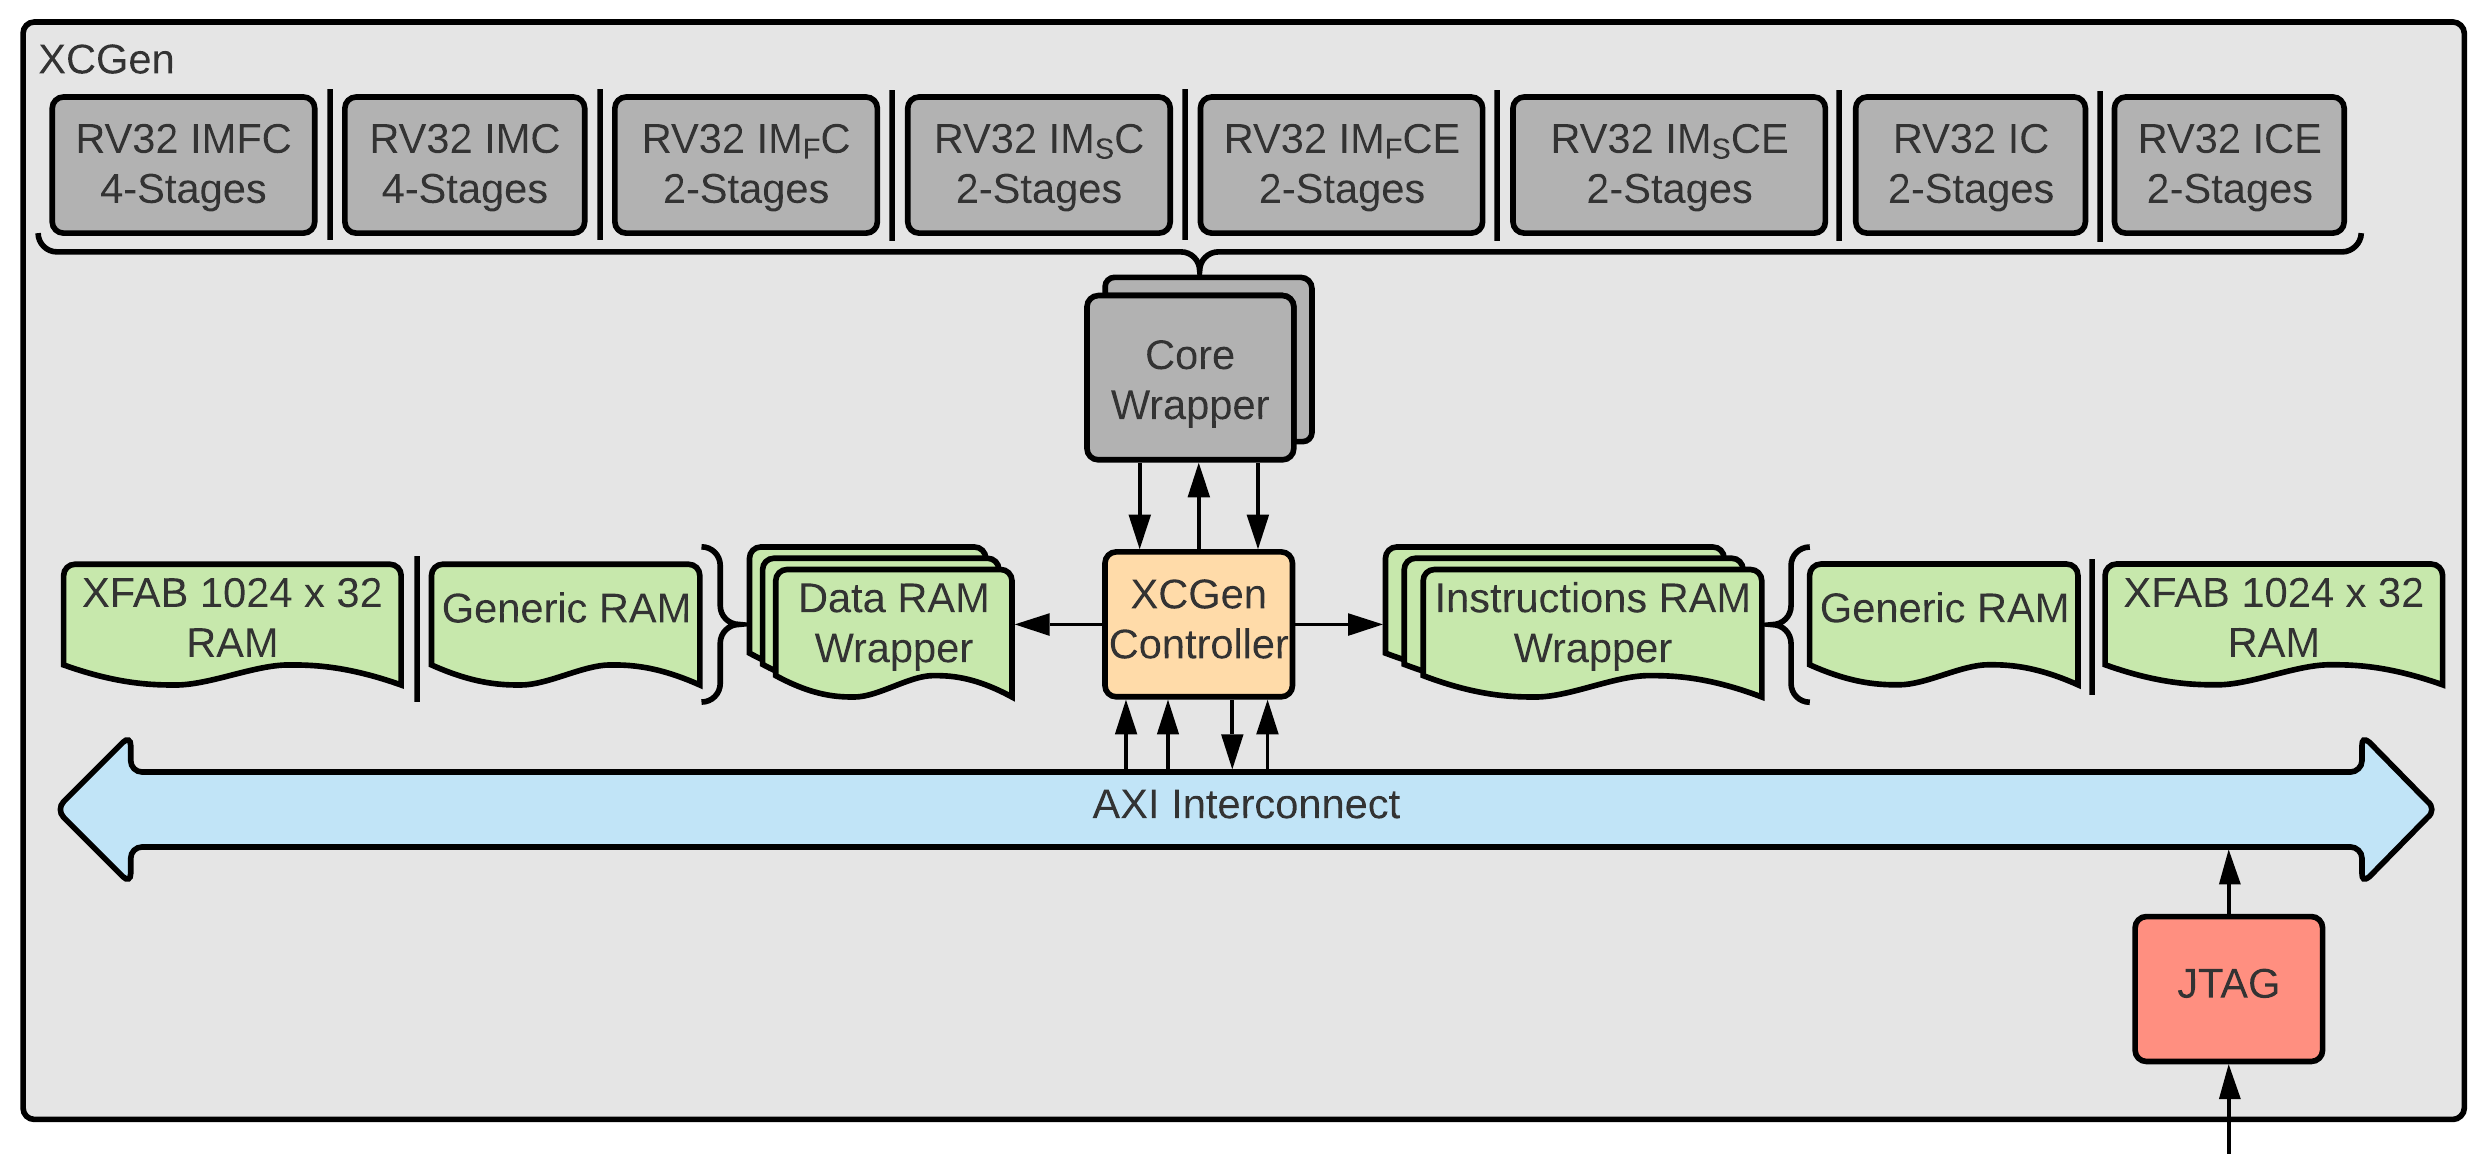
\includegraphics[width=\linewidth]{diagrams/XCGen2.png}
  \caption{Diagrama do XCGen.}
  \label{fig:top}
\end{figure}

\subsection{Visão Geral}
\label{sec:vgeral}
\par O XCGen consiste de um topo, feito na linguagem "System Verilog", onde é possível, através do uso de generates, adicionar ou remover blocos e alterar o mapa de memória na região de parametros do código.
Permitindo assim se ter novas funcionalidades e aplicações, através de um mesmo código, com o mínimo de alterações;
 \\
\par A arquitetura foi baseada no PULPINO o que permite o XCGen utilizra da ToolChain do RISC-V para geração de instruções em alto nível;

% section introdução (end)

